%% rnaastex.cls is the classfile used for Research Notes. It is derived
%% from aastex61.cls with a few tweaks to allow for the unique format required.
\documentclass[modern]{rnaastex}

\usepackage{graphicx}
\usepackage[suffix=]{epstopdf}
\usepackage{natbib}
\usepackage{amsmath}
\usepackage{xspace}
% make the word Kepler italicized, deal w/ floating space afterwards
\newcommand{\Kepler}{\textsl{Kepler}\xspace}


\begin{document}


\title{Searching for Transiting Exoplanets with NeoWISE}

%% Note that the corresponding author command and emails has to come
%% before everything else. Also place all the emails in the \email
%% command instead of using multiple \email calls.
\correspondingauthor{James. R. A. Davenport}
\email{jrad@uw.edu}

\author{James. R. A. Davenport}
\altaffiliation{NSF Astronomy and Astrophysics Postdoctoral Fellow; DIRAC Fellow}
\affiliation{Department of Physics \& Astronomy, Western Washington University, 516 High St., Bellingham, WA 98225, USA}
\affiliation{Department of Astronomy, University of Washington, Seattle, WA 98195, USA}


\author{Ethan Kruse}
\affiliation{Department of Astronomy, University of Washington, Seattle, WA 98195, USA}


%% Note that RNAAS manuscripts DO NOT have abstracts.
%% See the online documentation for the full list of available subject
%% keywords and the rules for their use.

%\keywords{SETI, asteroids, modeling?}


%%%%%%%
\section{} 

WISE and NeoWISE have a continuous viewing zone, meaning there is very dense light curves available for a small number of objects. indeed, WISE contains time series data for every object for many years, but usually only in small bursts every 6 months. Still, no comparable dataset exists for studying the variable sky at these wavelengths (W1=3.4, W2=4.6micron), and over these timescales.

WISE roll pattern means approx 90 min cadence for many years! the North/South Ecliptic Poles covered. South field has been studied vigorously with surveys such as OGLE (ref)

probably only a few hundred objects, given faint limits, colors, etc. That means we only expect order of 1 hot Jupiter for field stars.

In Figure \ref{fig:1} we show four example objects we have assembled of targets within the WISE CVZs with such densely sampled light curves, typically having $\sim$20,000 epochs of observation.

our search turned nothing conclusive up (TO SOME LIMIT?).  use Ethan/Eric's QATS code to look for transits. nothing... 

We write this Note to advertise WISE/NeoWISE as a unique data set for studying variability. Though the vast majority of stars do not have such dense sampling in WISE, essentially all targets will have regular visits, and a 7-year baseline.


\begin{figure*}[h!]
\begin{center}
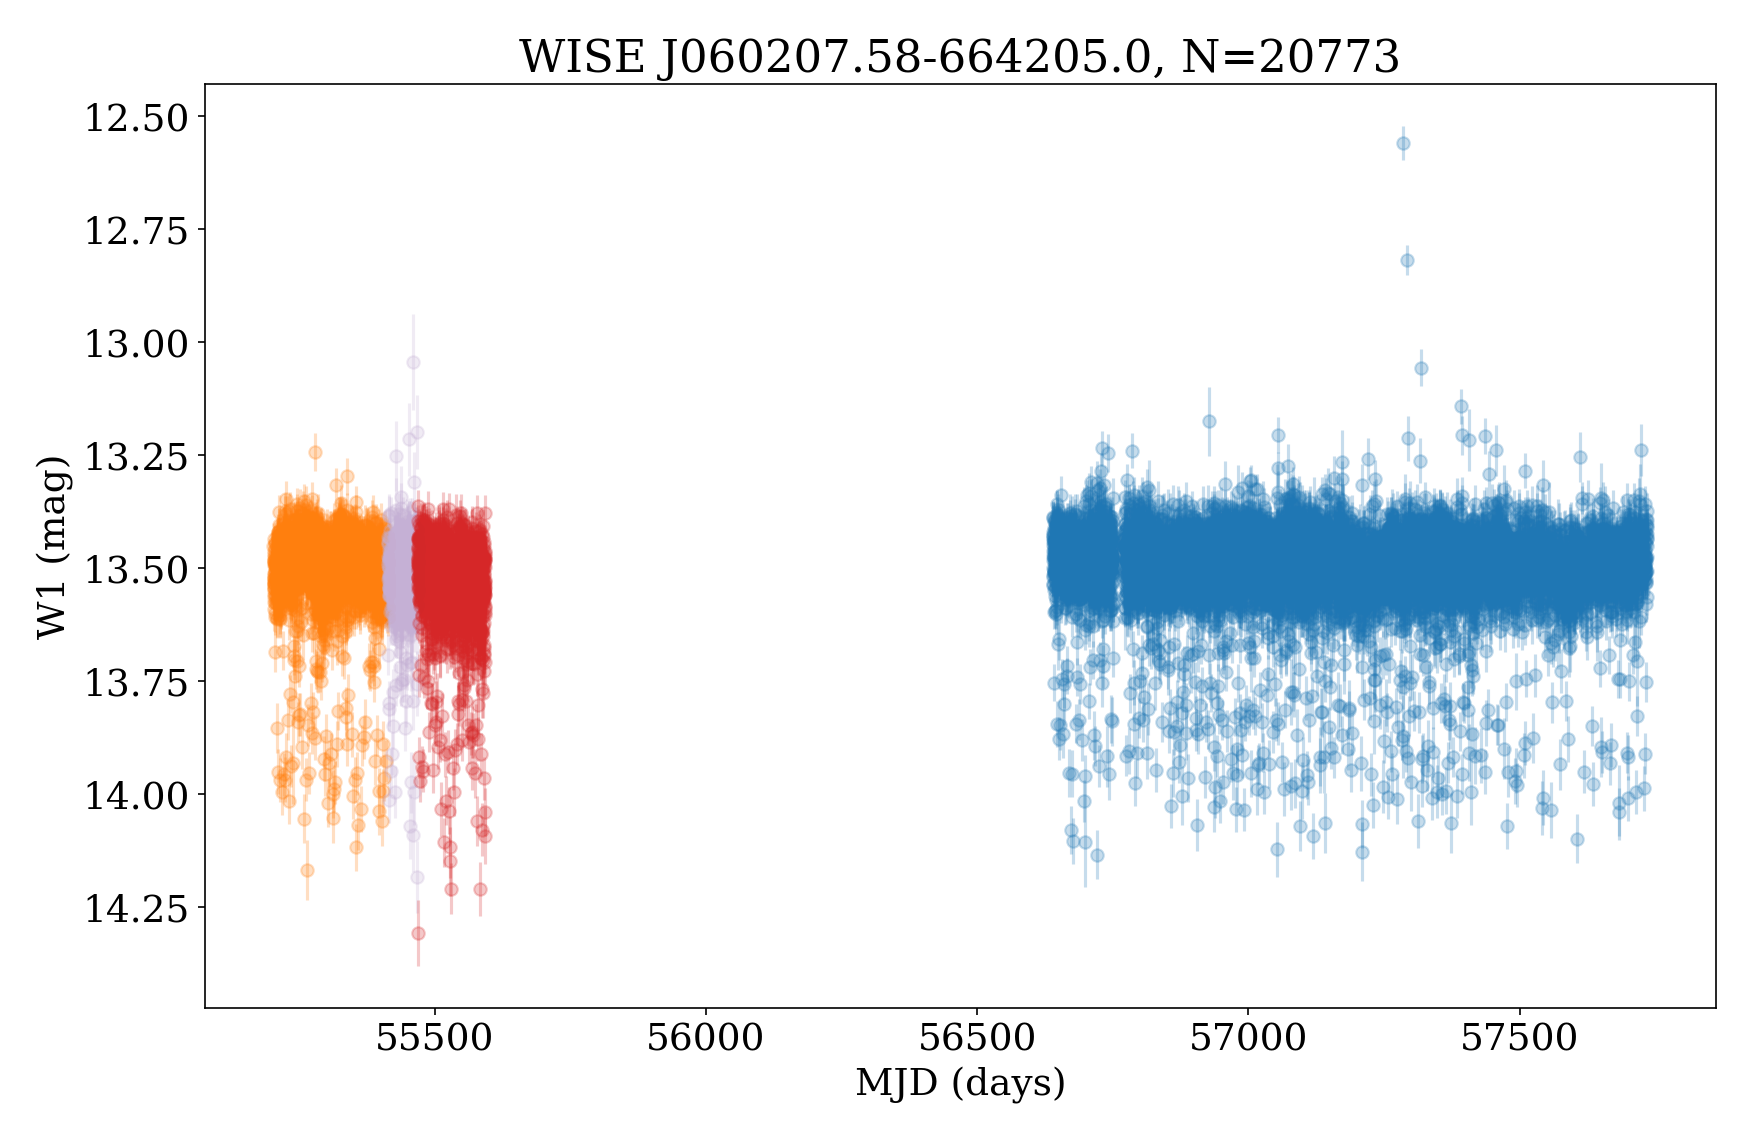
\includegraphics[width=3in]{img1a.png}
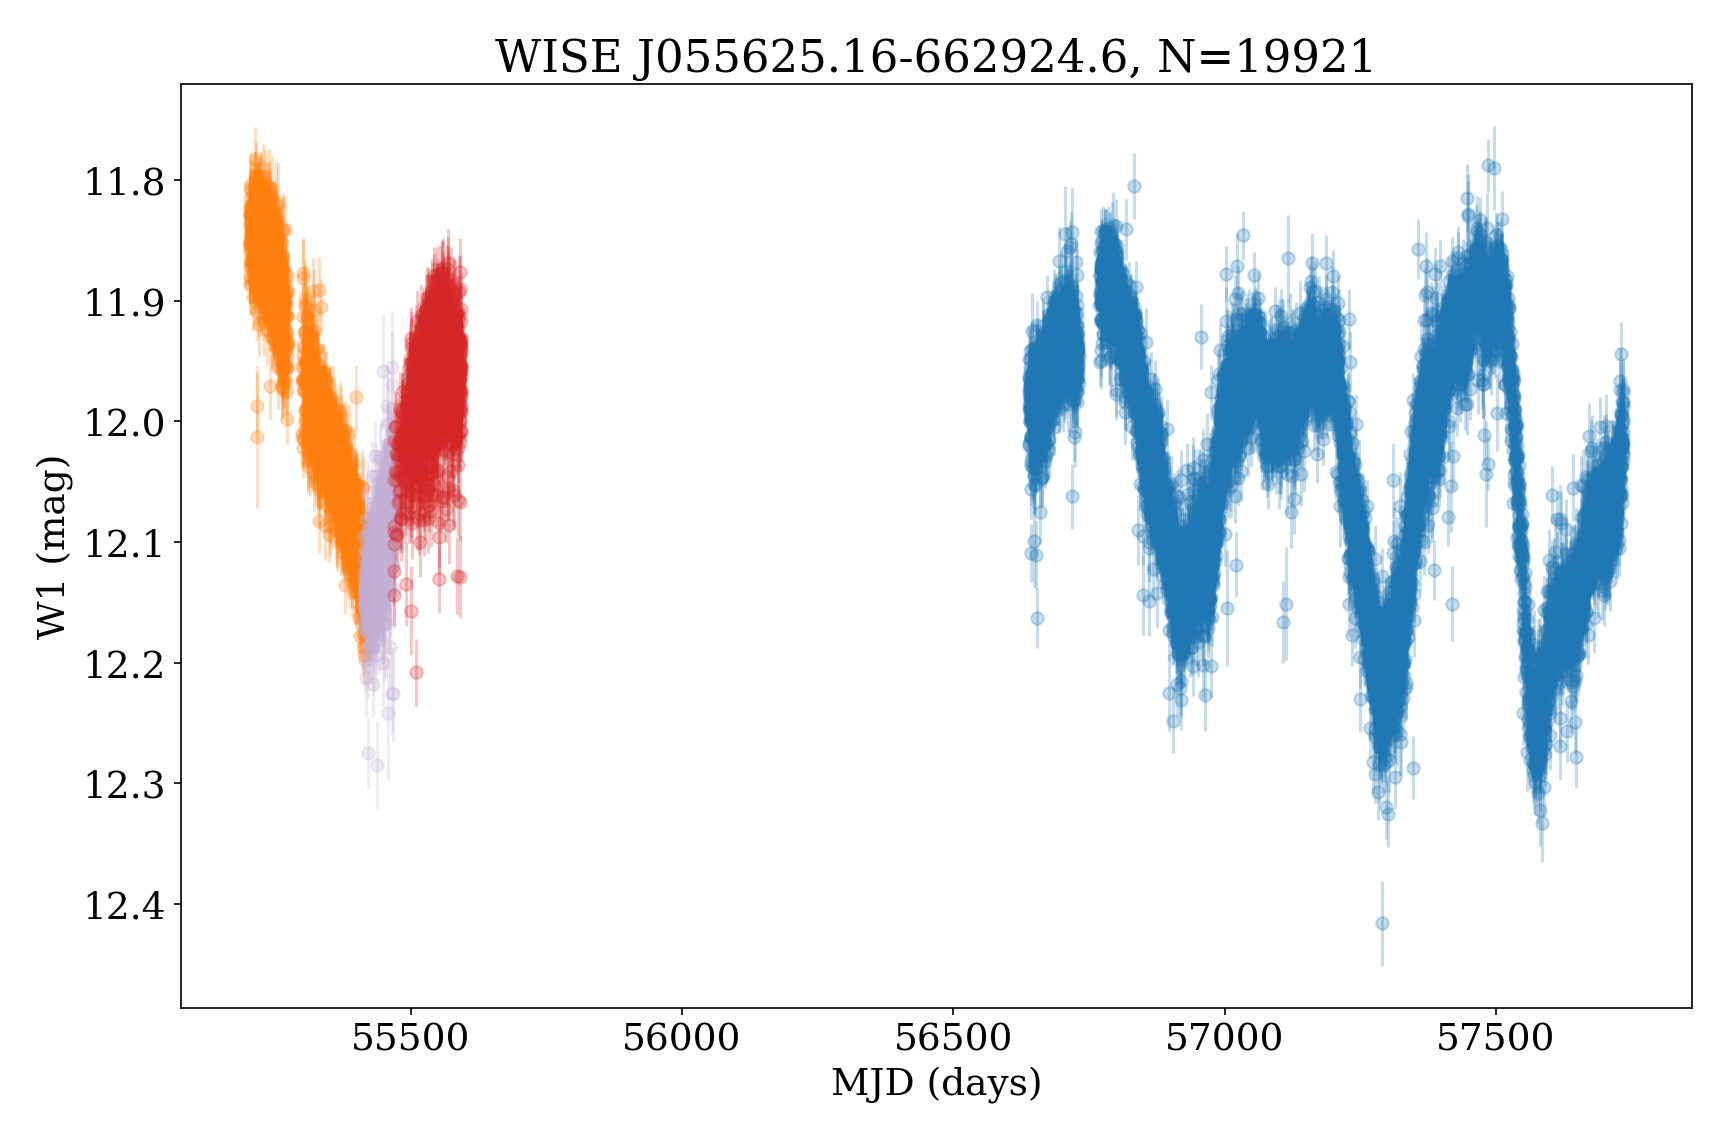
\includegraphics[width=3in]{img1b.png}\\
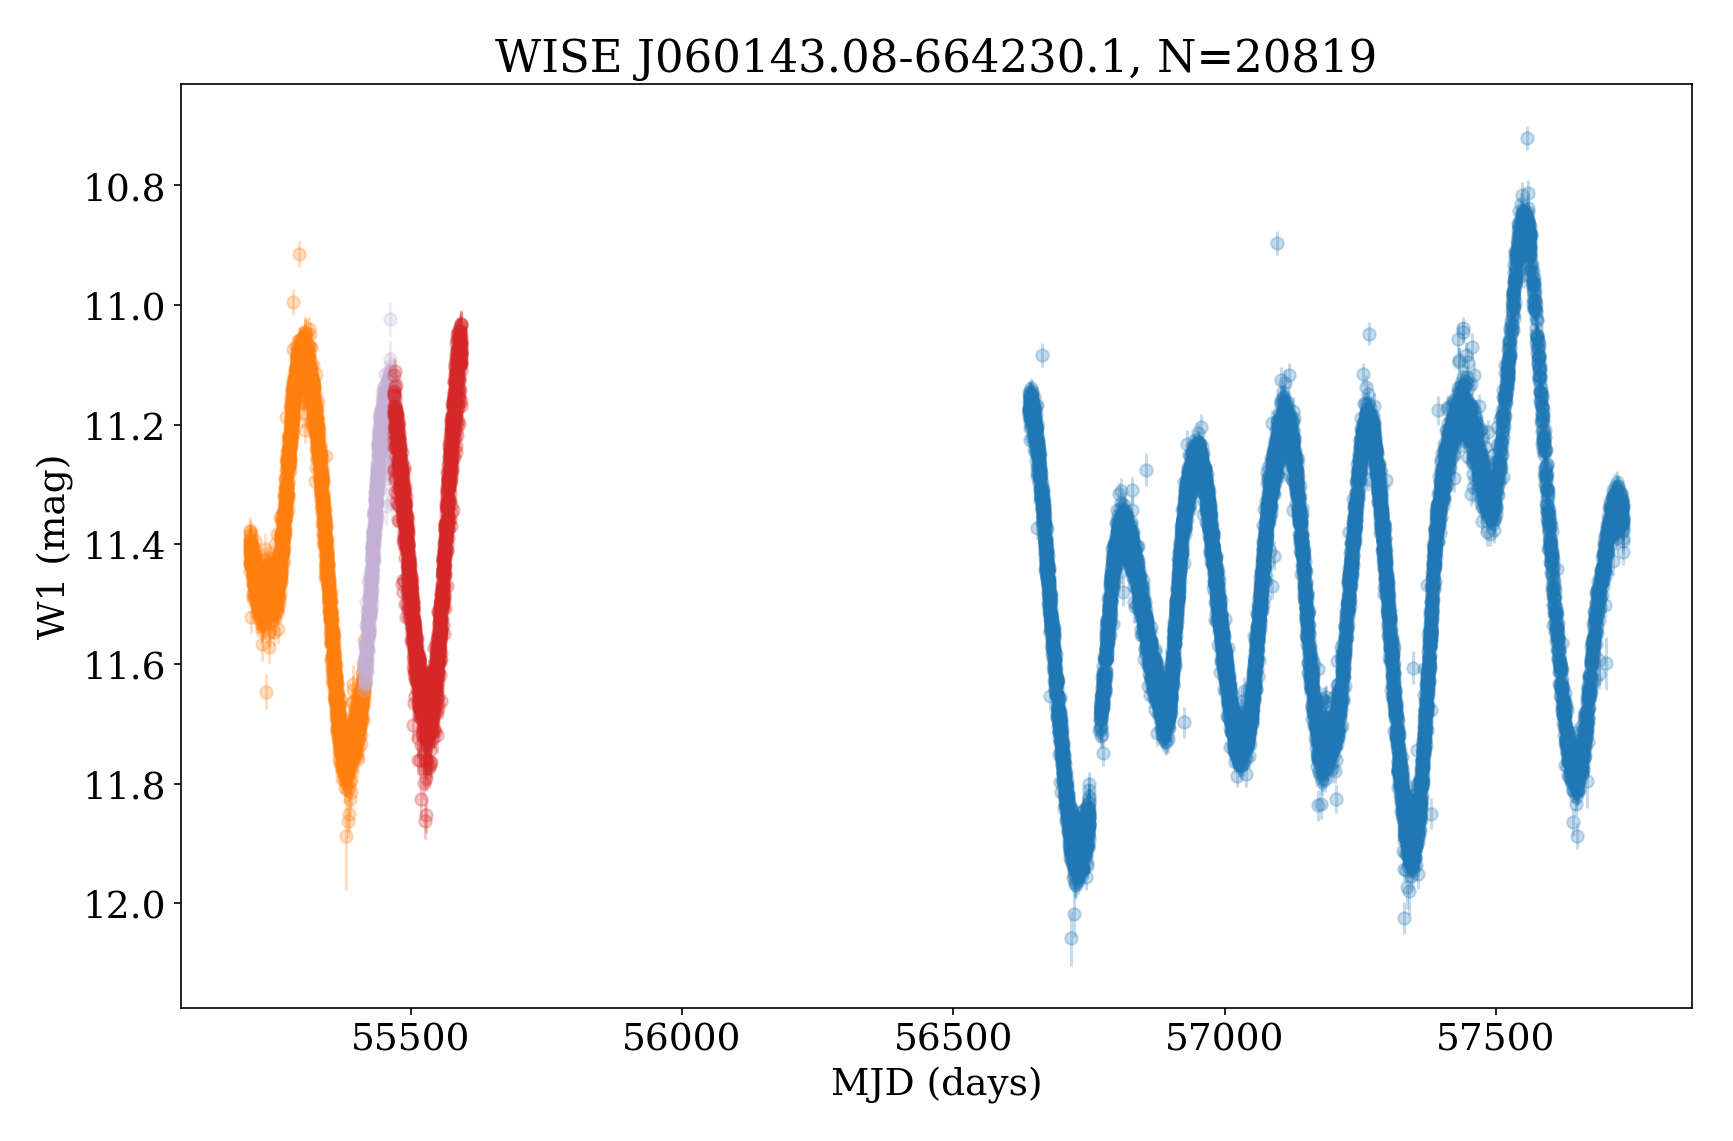
\includegraphics[width=3in]{img1c.png}
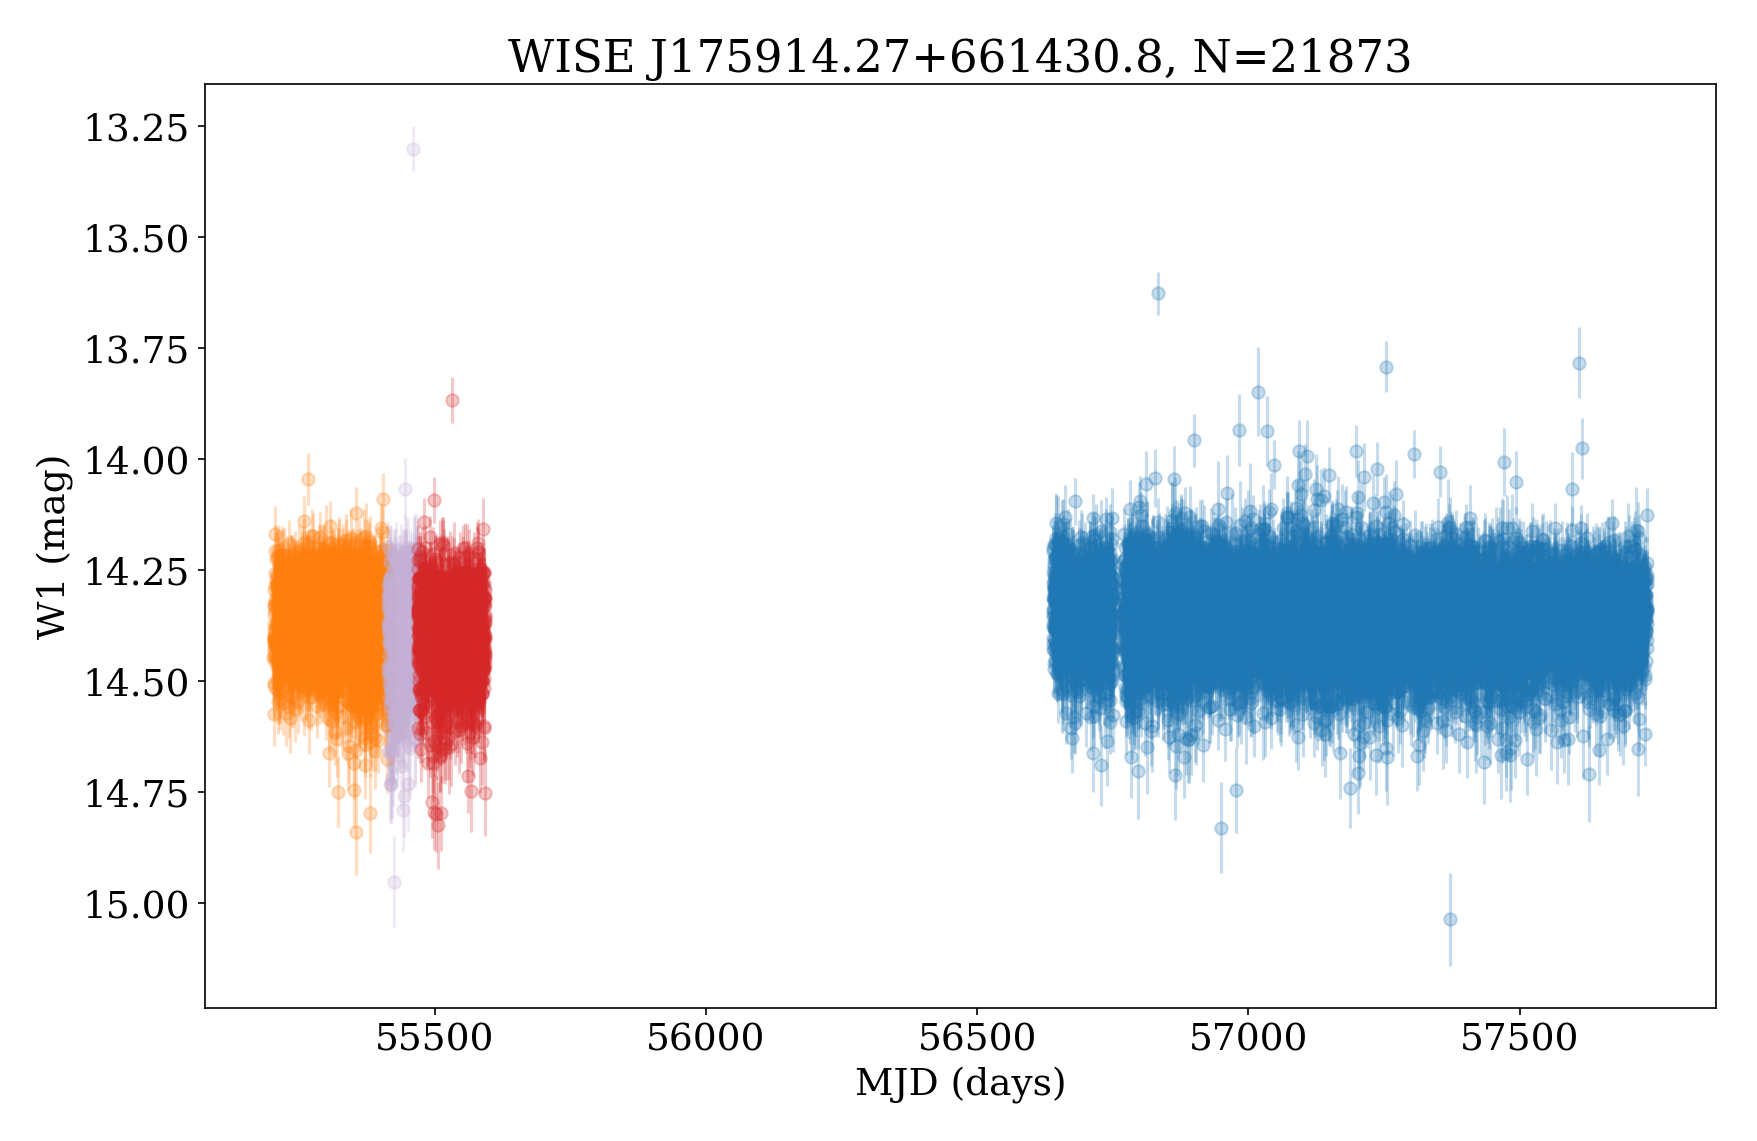
\includegraphics[width=3in]{img1d.png}
\caption{Four examples of light curves from the continuous viewing zones of WISE/NeoWISE, within about 50 arcmin of the Northern and Southern Ecliptic Poles. Data is colored by the WISE mission stage, including the original WISE data (orange points), WISE 3-band (light purple), WISE 2-band (red), and NeoWISE (blue). This set of light curves include a likely eclipsing binary (with X period?), two long period variable stars, and a photometrically quiet star. The vast majority of objects in this sample resemble the latter.
\label{fig:1}}
\end{center}
\end{figure*}


%%%%%%%%%
\acknowledgments

JRAD is supported by an NSF Astronomy and Astrophysics Postdoctoral Fellowship under award AST-1501418. 

The DIRAC Institute is supported through generous gifts from the Charles and Lisa Simonyi Fund for Arts and Sciences, and the Washington Research Foundation

%%%%%%%%%%%%%%%%%
\bibliography{/Users/james/Dropbox/references.bib}


\end{document}
